\section{Bayesian network}

A Bayesian network describes the joint probability distribution of variables using a directed graph. 
Nodes represent random variables, and edges indicate direct influence.
\begin{example}
    In the provided Bayesian network:
    \begin{figure}[H]
        \centering
        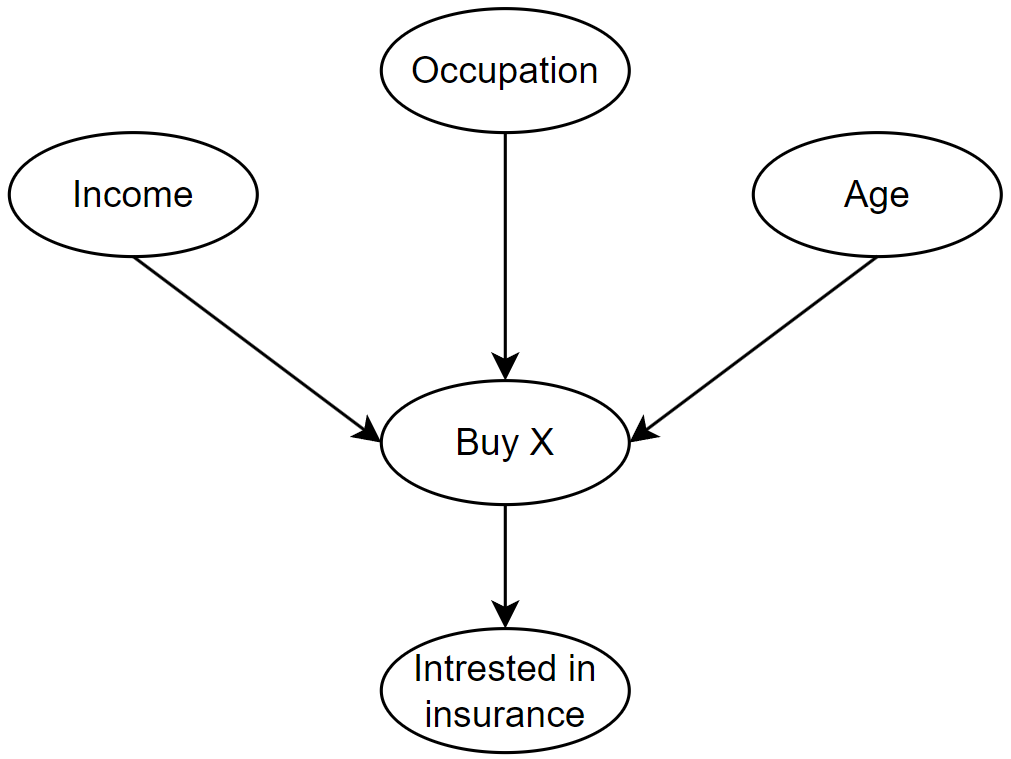
\includegraphics[width=0.4\linewidth]{images/insurance.png}
    \end{figure}
    Random variables "age," "income," and "occupation" are independent, whereas "buy X" and "Interested in insurance" are conditional probability distributions.
\end{example}
For a set of variables $x_1, x_2, \ldots, x_n$ we can determine any combination probability using a Bayesian network with $2^N - 1$ parameters. 
To represent these probabilities within the network, we require only the priors and conditional parameters. 
This is achieved by multiplying the number of nodes by $2^k$, where $k$ represents the number of incoming edges, giving us the total number of parameters needed.
\begin{example}
    In the provided Bayesian network:
    \begin{figure}[H]
        \centering
        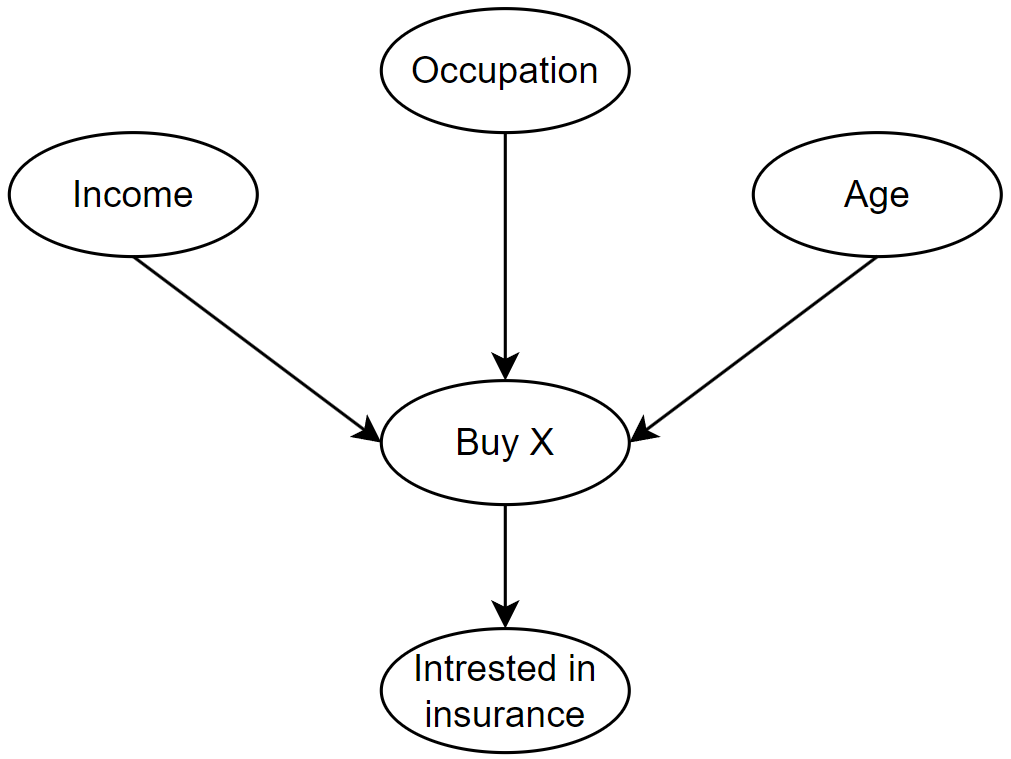
\includegraphics[width=0.4\linewidth]{images/insurance.png}
    \end{figure}
    For the full joint distribution, we require $2^N - 1$ parameters, which in this case is $2^5 - 1 = 31$ parameters.
    To represent the Bayesian network itself, we need to calculate the parameters required:
    \begin{itemize}
        \item For the "income", "occupation", and "age" nodes with no incoming edges: $3 \cdot 2^0 = 3$ parameters.
        \item For the "buy x" node with three incoming edges: $1 \cdot 2^3 = 8$ parameters.
        \item For the "Interested" node with one incoming edge: $1 \cdot 2^1 = 2$ parameters.
    \end{itemize}
    So, the total parameters needed to represent the Bayesian network is $3 + 8 + 2 = 13$ parameters.
\end{example}
\begin{definition}[\textit{Conditionally indipendent}]
    We define $X_1$ to be conditionally independent of $X_2$ given $X_3$ if the probability of $X_1$ is not influenced by the value of $X_2$ when we have knowledge about $X_3$.  
    This can be expressed as:
    \[\textnormal{P}(X_1|X_2,X_3)=\textnormal{P}(X_1|X_3)\]
\end{definition}
Likewise, for sets of variables, we can state that $X_1, X_2, X_3$ are independent of $Y_1, Y_2, Y_3$ given $Z_1,Z_2,Z_3$:
\[\textnormal{P}(X_1,X_2,X_3|Y_1,Y_2,Y_3,Z_1,Z_2,Z_3)=\textnormal{P}(X_1,X_2,X_3|Z_1,Z_2,Z_3)\]
\begin{example}
    Martin and Norman are tossing the same coin, and we have two variables: $A$ represents "Norman's outcome," and $B$ represents "Martin's outcome". 
    If the coin might be biased, $A$ and $B$ are not independent. 
    Observing that $B$ is heads leads us to revise our belief in $A$ being heads. 
    Therefore, we have:
    \[\textnormal{P}(A|B) \neq \textnormal{P}(A)\]
    Both variables $A$ and $B$ are dependent on another variable, $C$, representing "the coin is biased towards heads with probability $\theta$".
    Once we know the value of $C$, any evidence about $B$ cannot alter our belief about $A$.
    This can be expressed as:
    \[\textnormal{P}(A|B,C)=\textnormal{P}(A|C)\]
\end{example}
\begin{definition}[\textit{Prior probability}]
    A prior probability is a probability associated with a variable that has no incoming edges in a Bayesian network. 
\end{definition}
It's important to note that in a Bayesian network, a node is independent of its ancestors, given its parent node.
\begin{example}
    The event "grass is wet" ($W=true$) can be caused by two possible factors: either the "sprinkler" is on ($S=true$), or it is "raining" ($R=true$). 
    The corresponding Bayesian network is as follows.
    \begin{figure}[H]
        \centering
        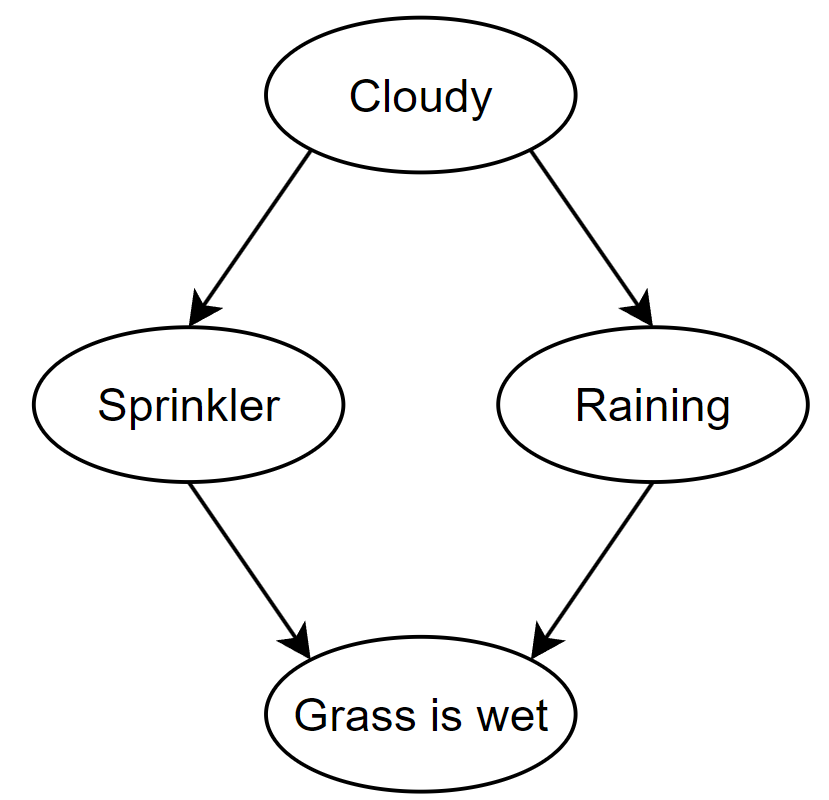
\includegraphics[width=0.25\linewidth]{images/sprinkler.png}
    \end{figure}
    Where the probabilities for cloudy are: 
    \begin{table}[H]
        \centering
        \begin{tabular}{cc}
        \hline
        \textbf{Cloudy} & \textbf{P(C)} \\ \hline
        0      & 0.5  \\
        1      & 0.5  \\ \hline
        \end{tabular}
    \end{table}
    Where the probabilities for sprinkler are: 
    \begin{table}[H]
        \centering
        \begin{tabular}{ccc}
        \hline
        \textbf{Sprinkler} & \textbf{Cloudy} & \textbf{P(S$|$C)} \\ \hline
        0         & 0      & 0.1  \\
        0         & 1      & 0.5  \\
        1         & 0      & 0.9  \\
        1         & 1      & 0.5  \\ \hline
        \end{tabular}
    \end{table}
    Where the probabilities for raining are: 
    \begin{table}[H]
        \centering
        \begin{tabular}{ccc}
        \hline
        \textbf{Raining} & \textbf{Cloudy} & \textbf{P(R$|$C)} \\ \hline
        0       & 0      & 0.8    \\
        0       & 1      & 0.5    \\
        1       & 0      & 0.2    \\
        1       & 1      & 0.5    \\ \hline
        \end{tabular}
    \end{table}
    Where the probabilities for the wet grass are: 
    \begin{table}[H]
        \centering
        \begin{tabular}{cccc}
        \hline
        \textbf{Wet} & \textbf{Sprinkler} & \textbf{Raining} & \textbf{P(W$|$S,R)} \\ \hline
        0            & 0                  & 0                & 1                   \\
        0            & 0                  & 1                & 0.1                 \\
        0            & 1                  & 0                & 0.1                 \\
        0            & 1                  & 1                & 0,01                \\
        1            & 0                  & 0                & 0                   \\
        1            & 0                  & 1                & 0.9                 \\
        1            & 1                  & 0                & 0.9                 \\
        1            & 1                  & 1                & 0.99                \\ \hline
        \end{tabular}
    \end{table}
    With all these values it is possible to compute all the probabilities with the formula: 
    \[
    \begin{aligned}
        \textnormal{P}(C,S,R,W)     &= \textnormal{P}(W|S,R,C)\textnormal{P}(S,R,C)=      \\
                                    &= \textnormal{P}(W|S,R)\textnormal{P}(S,R,C)=        \\
                                    &= \textnormal{P}(W|S,R)\textnormal{P}(S|R,C)P(R,C)=  \\
                                    &= \textnormal{P}(W|S,R)\textnormal{P}(S|C)P(R,C)=    \\
                                    &= \textnormal{P}(W|S,R)\textnormal{P}(S|C)P(R|C)P(C)
    \end{aligned}
    \]
    With this formula we can compute all the joint probabilities.
    \begin{table}[H]
        \centering
        \begin{tabular}{cccc|c}
        \hline
        \textbf{C} & \textbf{S} & \textbf{W} & \textbf{R} & \textbf{P(C, S, W, R)} \\ \hline
        0          & 0          & 0          & 0          & 0.04                \\
        0          & 0          & 0          & 1          & 0                   \\
        0          & 0          & 1          & 0          & 0.001               \\
        0          & 0          & 1          & 1          & 0.009               \\
        0          & 1          & 0          & 0          & 0.036               \\
        0          & 1          & 0          & 1          & 0.324               \\
        0          & 1          & 1          & 0          & 0.0009              \\
        0          & 1          & 1          & 1          & 0.0891              \\
        1          & 0          & 0          & 0          & 0.125               \\
        1          & 0          & 0          & 1          & 0                   \\
        1          & 0          & 1          & 0          & 0.0125              \\
        1          & 0          & 1          & 1          & 0.1125              \\
        1          & 1          & 0          & 0          & 0.125               \\
        1          & 1          & 0          & 1          & 0.1125              \\
        1          & 1          & 1          & 0          & 0.00125             \\
        1          & 1          & 1          & 1          & 0.12375             \\ \hline
        \end{tabular}
    \end{table}
\end{example}
In statistics, the phenomenon of explaining away is often referred to as Berkson's paradox or selection bias. It pertains to situations where two variables become dependent due to the observation of a third variable. 

\paragraph*{Classification}
In a Bayesian network, the relationships between variables can exhibit various types of dependencies and independencies: 
\begin{itemize}
    \item $\textnormal{P}(X,Y,Z)=\textnormal{P}(X)\textnormal{P}(Y)\textnormal{P}(Z|X,Y)$ and $\textnormal{P}(X,Y|Z)=\textnormal{P}(X)\textnormal{P}(Y)$ if the nodes are connected in the following way. 
        \begin{figure}[H]
            \centering
            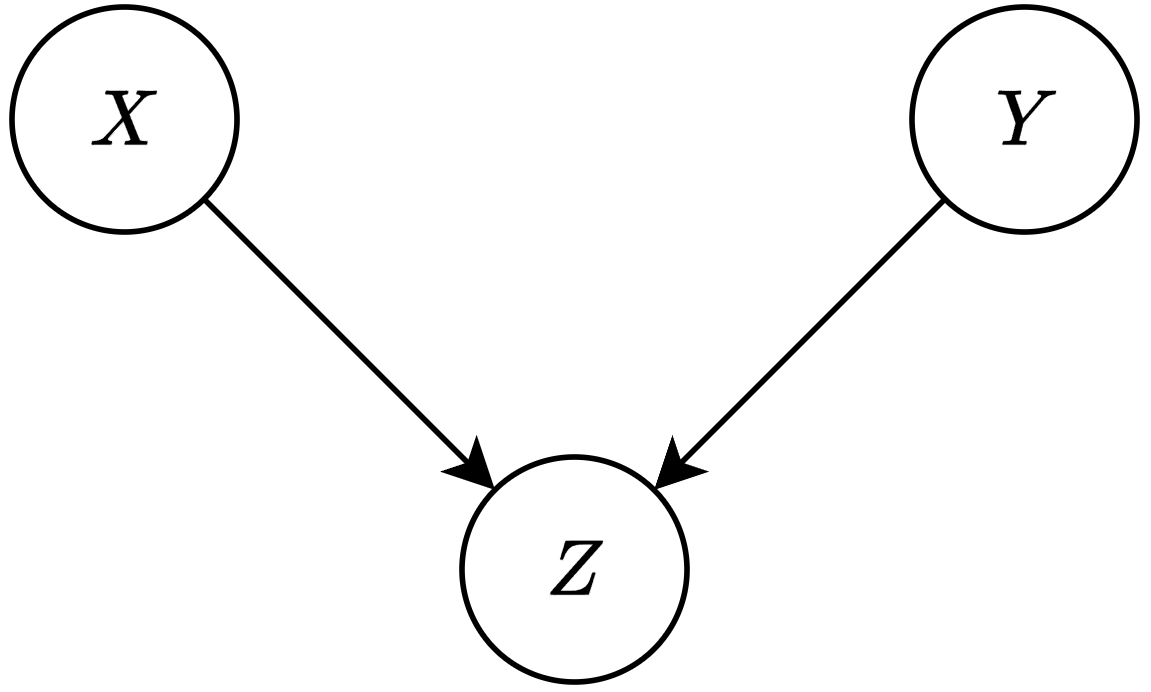
\includegraphics[width=0.3\linewidth]{images/independencies1.png}
        \end{figure}
    \item $\textnormal{P}(X,Y,Z)=\textnormal{P}(X|Z)\textnormal{P}(Y|Z)\textnormal{P}(Z)$ and $\textnormal{P}(X,Y|Z)=\textnormal{P}(X|Z)\textnormal{P}(Y|Z)$ if the nodes are connected in the following way. 
        \begin{figure}[H]
            \centering
            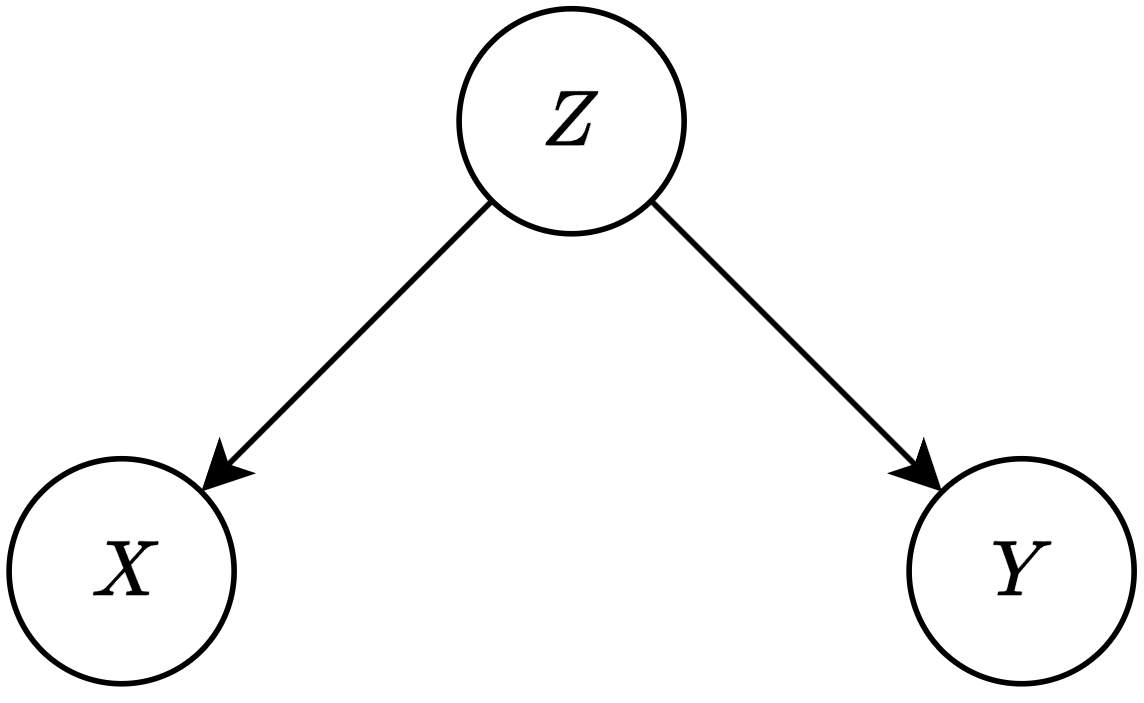
\includegraphics[width=0.3\linewidth]{images/independencies2.png}
        \end{figure}
    \item $\textnormal{P}(X,Y,Z)=\textnormal{P}(X)\textnormal{P}(Z|X)\textnormal{P}(Y|Z)$ and $\textnormal{P}(X,Y|Z)=\textnormal{P}(X|Z)\textnormal{P}(Y|Z)$ if the nodes are connected in the following way. 
        \begin{figure}[H]
            \centering
            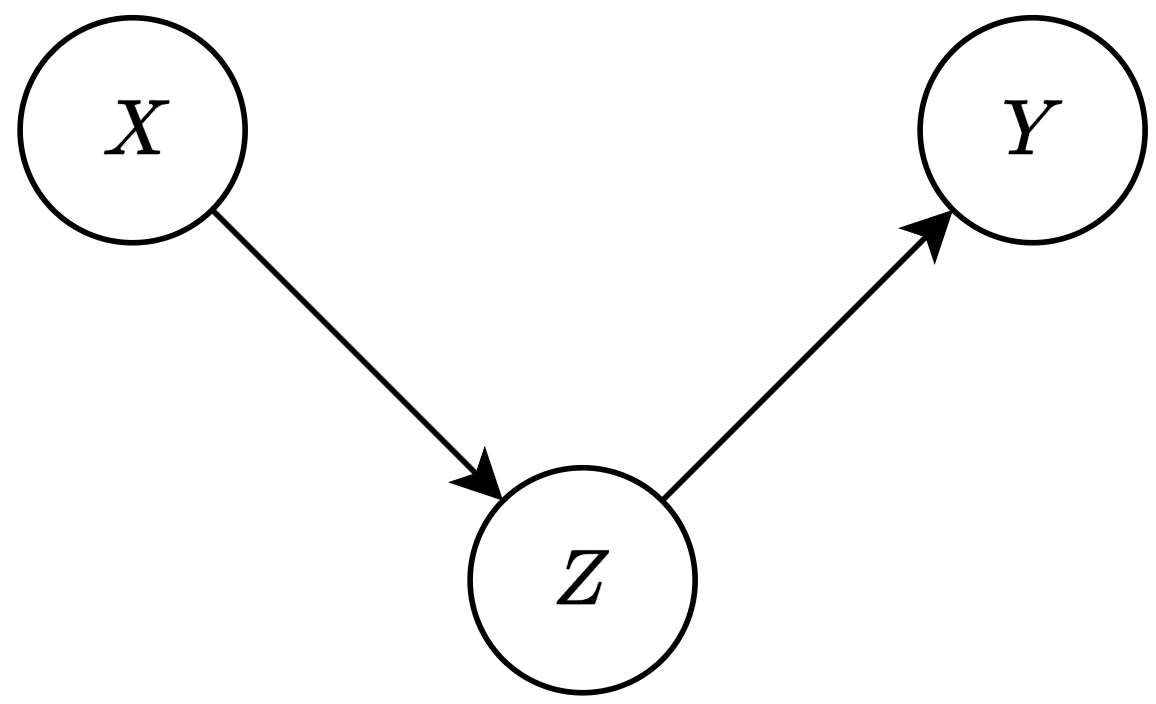
\includegraphics[width=0.3\linewidth]{images/independencies3.png}
        \end{figure}
\end{itemize}
\begin{definition}[\textit{Conditional indipendence}]
    Two sets of nodes, denoted as $A$ and $B$, exhibit what is termed as conditional independence or are often referred to as being d-separated, given a set of nodes $C$ if and only if all paths from $A$ to $B$ are effectively blocked by the presence of $C$.
\end{definition}
When we classify $C$ based on its role within a Bayesian network:
\begin{itemize}
    \item $C$ is categorized as a root when it remains hidden or unobserved. 
        In this scenario, the children of $C$ are dependent on each other due to the influence of a common unobserved cause. 
        However, if $C$ is observed, the children become conditionally independent, meaning that the common unobserved cause is no longer exerting an impact.
    \item $C$ is termed a leaf when it is hidden, and its parent nodes are marginally independent of one another. 
        Nevertheless, if $C$ (or any descendant of $C$) is observed, the parent nodes become dependent on each other, introducing conditional dependence.
    \item $C$ is described as a bridge when the nodes both upstream and downstream of $C$ become dependent solely when $C$ remains hidden. 
        Conditioning on $C$, by observing or introducing knowledge about it, effectively disrupts the graph's structure at that particular point, resulting in dependence between the nodes on either side of $C$.
\end{itemize}
These distinctions in the role of $C$ are essential in understanding how the presence or absence of observations can affect the conditional independence relationships within a Bayesian network.
\begin{figure}[H]
    \centering
    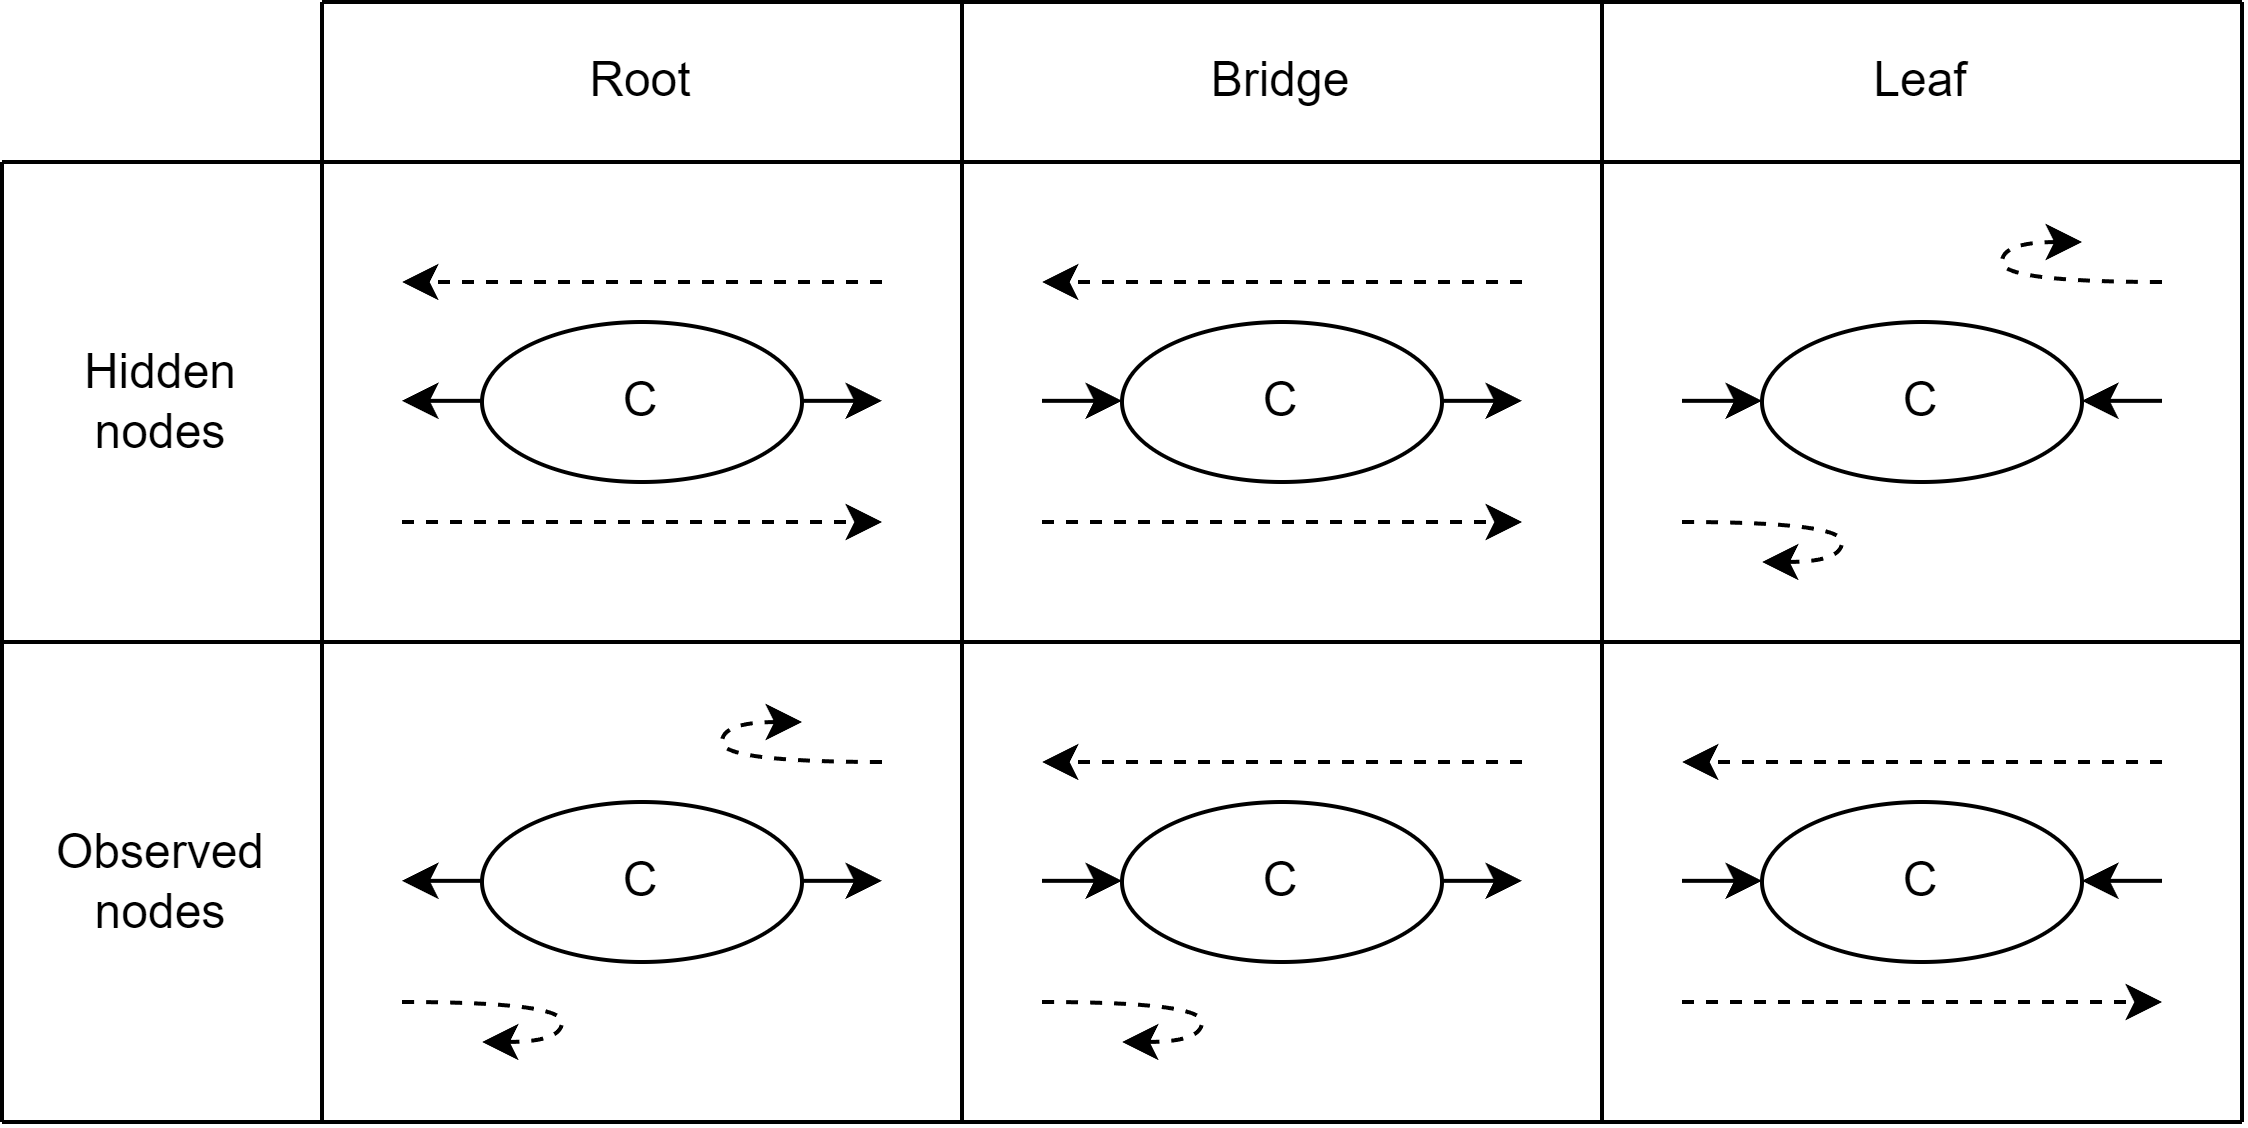
\includegraphics[width=0.75\linewidth]{images/def.png}
    \caption{Graphical representation of root, bridge, and leaf}
\end{figure}

\paragraph*{Bayesian networks reasoning}
Two distinct modes of reasoning are applicable when working with Bayesian networks:
\begin{itemize}
    \item \textit{Bottom-up reasoning}: this approach involves inferring the cause when provided with evidence. 
        In other words, it seeks to determine the underlying factors or causes that may have led to observed outcomes.
    \item \textit{Top-down reasoning}: in this mode, we calculate the probability of one event given another event. 
        This represents a predictive utilization of Bayesian networks, as they function as "generative" models. 
        It's about estimating the likelihood of certain events based on other known events.
\end{itemize}
One of the most intriguing attributes of Bayesian networks is their ability to facilitate causal reasoning grounded in a robust mathematical foundation. 
These networks allow us to explore and understand causal relationships within complex systems using a formal and structured approach.

Moreover, Bayesian networks can encompass nodes with both continuous (real) and discrete values. 
This versatility provides us with a diverse and powerful toolkit for constructing probabilistic models that can represent a wide range of real-world scenarios and phenomena.